\documentclass[11pt]{beamer}
\usetheme{Madrid}
\usepackage[utf8]{inputenc}
\usepackage{amsmath}
\usepackage{amsfonts}
\usepackage{amssymb}
\usepackage{graphicx}
\usepackage{mathptmx}
\usepackage{chancery}
\usepackage{wrapfig}
\usepackage{hyperref}

%\author{}
%\title{}
%\setbeamercovered{transparent} 
%\setbeamertemplate{navigation symbols}{} 
%\logo{} 
%\institute{} 
%\date{} 
%\subject{} 
\begin{document}

\begin{frame}

\begin{figure}[center]
  
\includegraphics[width=3.5cm, height=4cm]{Img/ULA.png}
\end{figure}


{\bf \large Nombre  :} \large HUALLPAR DORADO, Jhoel \\
{\bf \large Curso   :} \large Estructura de Datos \\
{\bf \large Docente :} \large Luciano Arnaldo Romero Calla \\
{\bf \large Tema    :} \Large Fibonacci Heap\\
{\bf \large Correo  :} \large jhuallpard@ulasalle.edu.pe\\

\titlepage
\end{frame}

\begin{frame} {\bf \large \rightline{Fibonacci Heap   *}}
\tableofcontents
{\center \bf \Huge \color{purple} \texttt{FIBONACCI HEAP} \\}

\begin{figure}[center]
  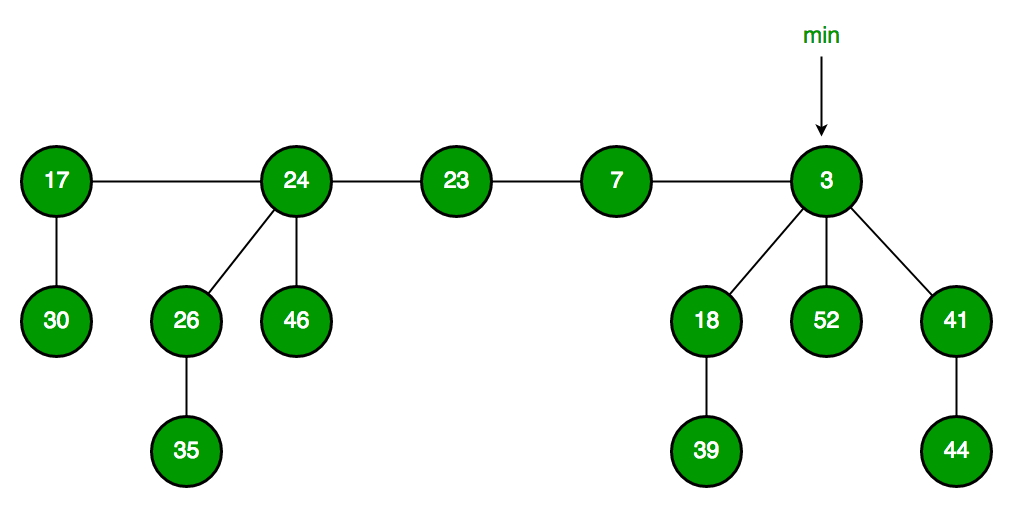
\includegraphics[width=10cm, height=5cm]{Img/FH.png}
\end{figure}

\end{frame}

\begin{frame} {\bf \large \rightline{Fibonacci Heap   *}}
\tableofcontents
{\center \bf \Large \color{red} CONTENIDO \\}

\begin{enumerate}
\item Introducci\'on
\item Insert
\item Extract Minimal or Delete Minimun
\item Find Minimun
\item Conclusi\'on
\item Referencias
\item Demo
\end{enumerate}

\end{frame}

\begin{frame}{\bf \large \rightline{Fibonacci Heap   *}}

{\center \bf \large \color{red} INTRODUCCI\'ON \\}

\begin{figure}[center]
  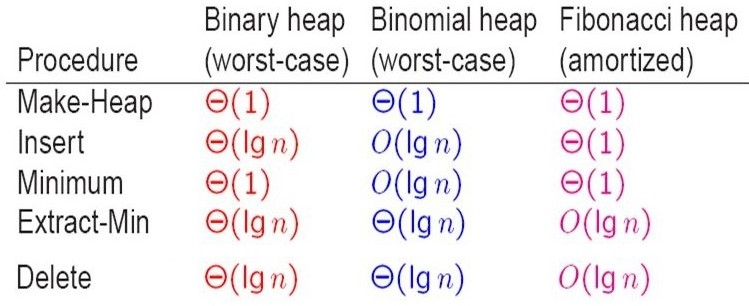
\includegraphics[width=7cm, height=3cm]{Img/Coste.jpg}
\end{figure}

	Se utiliza para mejorar el tiempo de ejecución asintótico del algoritmo de {\large Dijkstra}  {\bf "calcula el camino más corto en un grafo"} y el algoritmo de {\large Prim}  {\bf "calcula el árbol mínimo de un grafo"}.

\end{frame}

\begin{frame}{\bf \large \rightline{Fibonacci Heap   *}}

{\center \bf \large \color{red} INSERT \\}
	Buscar el elemento de valor mínimo:
El nodo de clave minima es precisamente el apuntado por M.min
El costo de esta operación es de O(1)\\

\begin{figure}[center]

  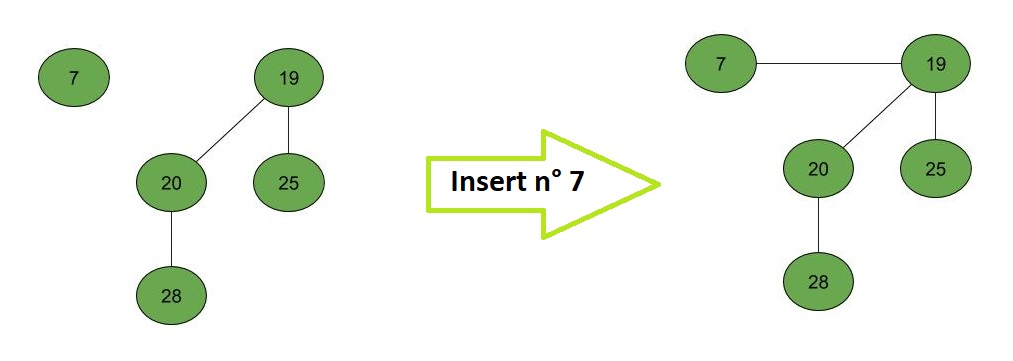
\includegraphics[width=12cm, height=5cm]{Img/Insert.jpg}
  
\end{figure}
\end{frame}

\begin{frame}{\bf \large \rightline{Fibonacci Heap   *}}

{\center \bf \large \color{red} Extract Minimal or Delete Minimal \\}
	{\bf Buscar el elemento de valor mínimo:}\\
	* El nodo con la clave m\'inima es precisamente el apuntado por M.min \\
	* El costo de esta operación es de {\bf O(1)}
	
\begin{figure}[center]
  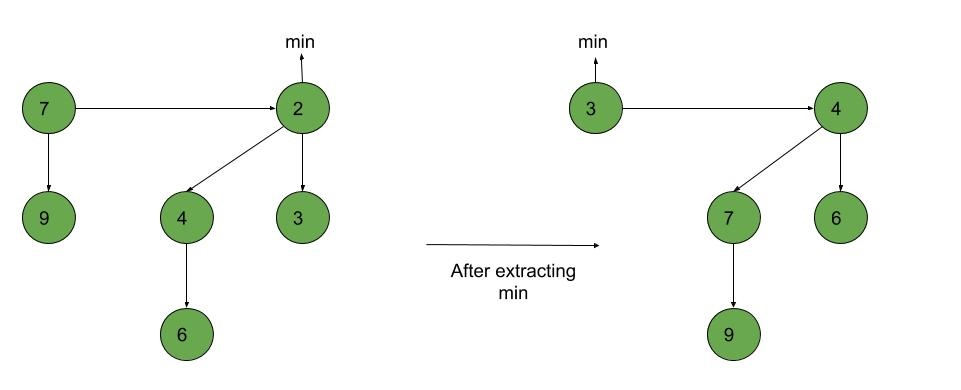
\includegraphics[width=12cm, height=4.5cm]{Img/EMinimo.jpg}
\end{figure}
\end{frame}

\begin{frame}{\bf \large \rightline{Fibonacci Heap   *}}

{\center \bf \large \color{red} Find Minimun \\}
\begin{figure}[center]
	La operación {\bf Encontrar Mínimo} es trivial porque guardamos el puntero al nodo que lo contiene.
  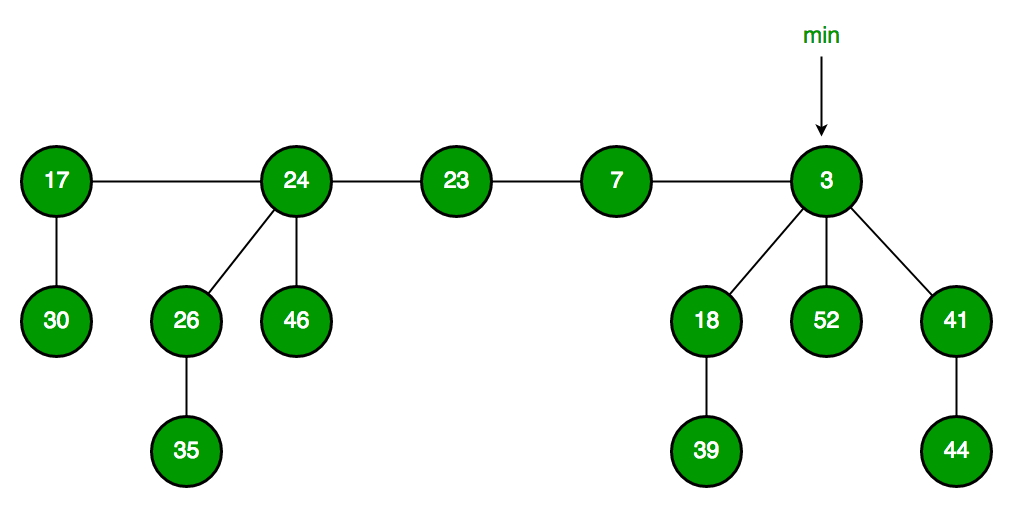
\includegraphics[width=10cm, height=4.5cm]{Img/BMinimo.png}
\end{figure}

\end{frame}

\begin{frame}{\bf \large \rightline{Fibonacci Heap   *}}

{\center \bf \huge \color{red} Conclusi\'on \\}

	* Fibonacci Heap es una estructura de datos que consiste en una colección de árboles.\\
	* Dispone de una mejor relación entre el coste y su amortización que el Binomial Heap.\\
	* Se denomina Fibonacci Heap principalmente porque los números de Fibonacci se utilizan en el análisis del tiempo de ejecución.\\
	* Aunque Fibonacci Heap parece ser de una complejidad de tiempo prometedora, en la práctica se ha encontrado lenta, ya que las constantes ocultas son altas.\\
\end{frame}

\begin{frame}{\bf \large \rightline{Fibonacci Heap   *}}

{\center \bf \huge \color{red} Referencias \\}

\begin{enumerate}
\item \href{https://www.cs.usfca.edu/~galles/JavascriptVisual/FibonacciHeap.html}{\scriptsize \color{blue} \underline{https://www.cs.usfca.edu/~galles/JavascriptVisual/FibonacciHeap.html}}\\

\item \href{https://www.geeksforgeeks.org/fibonacci-heap-set-1-introduction/}{\scriptsize \color{blue} \underline{https://www.geeksforgeeks.org/fibonacci-heap-set-1-introduction/}}\\

\item \href{https://www.slideshare.net/smarthur/expo-fibonacci}{\scriptsize \color{blue} \underline{https://www.slideshare.net/smarthur/expo-fibonacci}}\\

\item \href{http://web.karabuk.edu.tr/hakankutucu/CME222/MIT[1].Press.Introduction.to.Algorithms.2nd.Edition.eBook-TLFeBOOK.pdf}{\scriptsize \color{blue} \underline{Press Introduction to Algorithms 2nd Edition}}\\

\item \href{https://www.youtube.com/watch?v=mnIBSMvNSBk}{\scriptsize \color{blue} \underline{https://www.youtube.com/watch?v=mnIBSMvNSBk}}\\

\item \href{https://www.youtube.com/watch?v=tpmiDdMllg8}{\scriptsize \color{blue} \underline{https://www.youtube.com/watch?v=tpmiDdMllg8}}\\
	
\end{enumerate}

\begin{figure}[center]
  
\includegraphics[width=5cm, height=2.5cm]{Img/Referencias.jpg}
\end{figure}	
\end{frame}

\begin{frame}{\bf \large \rightline{Fibonacci Heap   *}}

{\center \bf \Large \color{red} Demo \\}
\begin{figure}[center]

  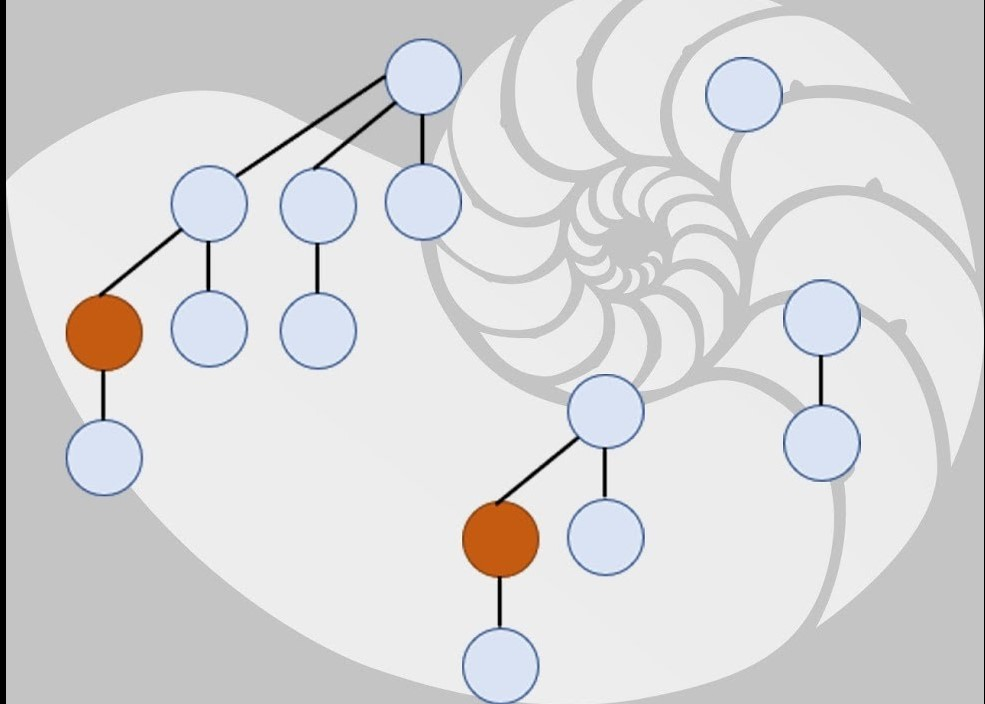
\includegraphics[width=10cm, height=6cm]{Img/Demo.jpg}
  
\end{figure}
\end{frame}

\begin{frame}{\bf \large \rightline{Fibonacci Heap   *}}

{\center \bf \Huge \color{purple} FINAL!!! \\}
\begin{figure}[center]

  
\includegraphics[width=9cm, height=6cm]{Img/Gracias.jpg}
  
\end{figure}
\end{frame}
\end{document}